\documentclass{report}
\usepackage[a4paper,margin=1in]{geometry}
\usepackage{fancyhdr}
\usepackage[titles]{tocloft}
\usepackage{tikz}
\usepackage{xcolor}

\usepackage{multicol}
\usepackage{amsmath}
\usepackage{amssymb}
\usepackage{pdfpages}
%\usepackage{biblatex}
%\addbibresource{bib.bib}

%hyperref should be last apparently
\usepackage{hyperref}

\renewcommand\cftsecdotsep{\cftdot}
\renewcommand\cftsubsecdotsep{\cftdot}

\newcommand{\tbf}{\textbf}

\newcommand*{\newpar}{\par\vspace{\baselineskip}\noindent} %start new unindented paragraph with empty line inbetween

\pagestyle{fancy} %allows headers

\lhead{Emma Bach}
\rhead{\today}

\renewcommand*\contentsname{Table of contents}


\begin{document}
\begin{titlepage}
	\centering
	{\Large \textsc{Study Notes}\par}
	\vspace{0.5cm}
	{\huge\bfseries Handbook of Logic in Computer Science\par}
    \vspace{1cm}
	{\Large\itshape Emma Bach\par}

% Bottom of the page
	{\large \today\par}
\end{titlepage}

\tableofcontents
\thispagestyle{fancy}
\chapter{Introduction}
\thispagestyle{fancy}
\section{Definition}
There is no fully rigorous 'mathematical' definition that cleanly seperates everything that is an embedded system from everything that isn't. Instead, embedded systems exist on a spectrum. We can say that a system is \textit{more embedded} or \textit{less embedded} depending on how many of the typical properties of an embedded system apply to it. \tbf{Embedded Systems} are \tbf{computer systems} that tend to:
\begin{itemize}
    \item be \tbf{integrated (embedded) into a larger system}, which they may control and/or provide information processing for.
    \item be \tbf{specialized} to provide exactly the functions they need to.
    \item be forced to work with \tbf{constraints} in time, memory, energy consumption, space, etc.
\end{itemize}
The term \tbf{Cyber-Physical System} generally refers to a larger system that combines computational elements with physical elements, with embedded systems generally being smaller components of such a system.
Examples of Cyber-Physical Systems include \tbf{IoT} (Internet of Things) devices, \tbf{Ubiquitous Computing} devices, and \tbf{SCADA} (Supervisory Control and Data Acquisition) systems.
\newpar
An embedded system generally consists of physical components such as sensors and actuators, computational components including memory and processors, and software. Since the computational components tend to work with digital representation of numbers, while the physical components work with analog voltages, additional conversion through A/D and D/A converters is needed.

\begin{figure}[h!]
\centering

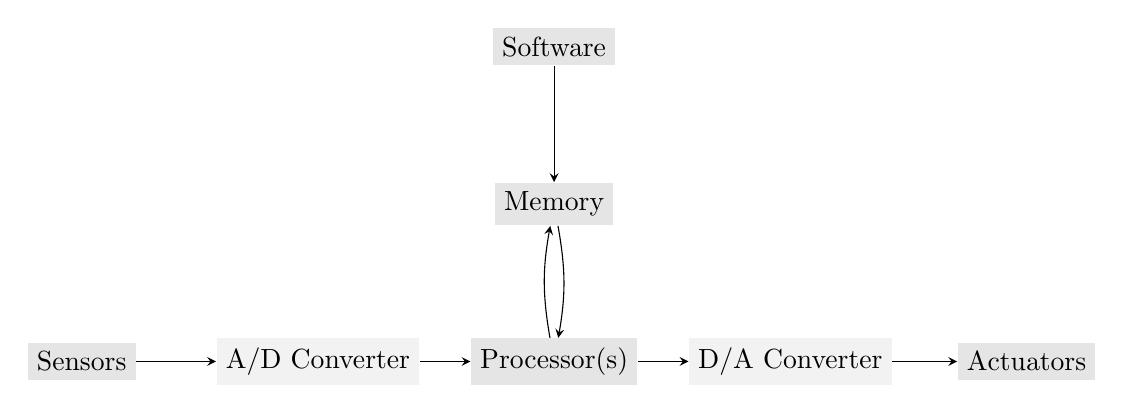
\begin{tikzpicture}[scale=1,-stealth]
\draw[fill=white!90!black] (0,0) node[fill](SE) {Sensors};

\draw[fill=white!95!black] (3,0) node[fill](AD) {A/D Converter};

\draw[fill=white!90!black] (6,0) node[fill](PR) {Processor(s)};
\draw[fill=white!90!black] (6,2) node[fill](ME) {Memory};
\draw[fill=white!90!black] (6,4) node[fill](SO) {Software};

\draw[fill=white!95!black] (9,0) node[fill](DA) {D/A Converter};

\draw[fill=white!90!black] (12,0) node[fill](AC) {Actuators};

\draw (SE) to (AD);
\draw (AD) to (PR);
\draw (SO) to (ME);
\draw (PR) to[bend left=10] (ME);
\draw (ME) to[bend left=10] (PR);
\draw (PR) to (DA);
\draw (DA) to (AC);

\end{tikzpicture}
\caption{The structure of a typical embedded system.}
\label{fig:embeddedsystemstructure}
\end{figure}

\newpar
Embedded systems have extremely widespread applications, especially in fields such as automotive and aerospace engineering and in medical technology.
%
\section{Design}
Embedded systems must be \tbf{dependable}:
\begin{itemize}
    \item The \tbf{Availability} is the probability of the system working at time t.
    \item The \tbf{Reliability} of an embedded system is the probability of the system working correctly provided that it was working at time t=0.
    \item The \tbf{Maintainability} is the probability of the system working correctly at time t+d after encountering an error at time t.
    \item Additional factors are \tbf{Safety} (How much harm could the system potentially cause?) and \tbf{Security} (How resistant to outside interference is the system?)
\end{itemize}
Since embedded systems are often employed in safety-critical roles, such as in the aforementioned aerospace industry, dependability is extremely important. For safety-critical systems, \tbf{redundancy} is generally a desired trait, so that if one component fails there are still other components to cover the same function.
\newpar
Embedded systems also generally need to be efficient enough to meet constraints in:
\begin{multicols}{2}
\begin{itemize}
    \item Energy consumption
    \item Physical Size
    \item Code Size
    \item Required Memory
    \item Runtime
    \item Weight
    \item Cost
    \item[\vspace{\fill}]
\end{itemize}
\end{multicols}
\newpar
Lastly, Embedded systems are typically \tbf{reactive systems}, meaning that they work through interacting with their environment at a pace dictated by that environment. This often also makes them \tbf{real-time systems}, meaning they need to meet real-time constraints - If a right answer arrives too late, it is just as bad as a wrong answer. If failure to meet a deadline results in catastrophe, that constrained is called a \tbf{hard constraint}. This means that worse average runtimes are acceptable, or even necessary, if it leads to a better worst case runtime. 
%
\chapter{Specification}
\thispagestyle{fancy}
Design by Contract (\tbf{DbC}), also known as contract programming or simply as internal testing, is the idea that software designers should define precise, formal, verifiable specifications for the desired behaviour of their systems. These often extend the ordinary usage of abstract data types with the description of desired preconditions, postconditions and invariants. The first steps of designing a system thus come down to translating the requirements of the project from natural language into a formal specification that verifiably meets the desired goals.
\newpar
Such specifications generally involve the \tbf{abstraction} of a given system in order to simplify its description, and hierarchical separation of the description, in order to make a description more easily digestible. We distinguish between two kinds of hierarchy:
\begin{itemize}
    \item Behavioral hierarchy, which describes a systems behavior in terms of states, events, and output signals. Examples of concepts of "high level" behavioral hierarchy are interrupts and exceptions.
    \item Structural hierarchy, which describes how a system can be thought of as a collection of seperate components: processors, actuators, sensors, etc.
\end{itemize}
Specifications generally need to describe a systems \tbf{Timing Behavior}, especially in the case of real-time systems. This involves specifying the elapsed time during execution of a given task, the delay between processes, Timeouts (maximum waiting times for a given event), and Deadlines.
\newpar
It is helpful to model a system as a flow of states (\tbf{State-Oriented Behavior}). However, classical automata are often insufficient, since they don't model timing and don't support hierarchical description. Common traits that a specification has to be able to model are:
\begin{itemize}
 \item Event-handling for both internal and external events (preferably supporting exception-oriented behavior)
 \item Modeling of concurrency
 \item Modeling of communication between different systems. Different models include:
 \begin{itemize}
  \item Synchronous communication ($A$ sends information directly to $B$)
  \item Asynchronous communication ($A$ writes to a buffer, the information is later sent to $B$)
  \item $A$ and $B$ write to and read from shared memory
 \end{itemize}
\end{itemize}
In order to qualify as a formal specification in the first place, naturally the specification needs to also have unambiguous semantics that support formal verification.
%
\section{Automaton Models}
%
\subsection{State Machines}
As a reminder: a \tbf{finite state machine (FSM)}, also known as a \tbf{deterministic finite automaton (DFA)}, is a tuple $M = (I, S, s_0, \delta, F)$, such that:
\begin{itemize}
 \item $I$ is a finite, non-empty set, called the set of input \tbf{symbols}
 \item $S$ is a finite, non-empty set, called the set of \tbf{states}
 \item $s_0 \in S$ is called the \tbf{initial state}
 \item $\delta$ is a function $S \times I \to S$, called the \tbf{\colorbox{cyan}{\strut t}\colorbox{pink}{\strut r}\colorbox{white}{\strut a}\colorbox{pink}{\strut n}\colorbox{cyan}{\strut s}ition function}
 \item $F \subseteq S$ is called the set of \tbf{final states} or \tbf{accepting states}
\end{itemize}
As a computer science student, I myself was already very comfortable working with DFAs before this lecture, and I will thus skip the basic explanations of the topic.
\newpar
One major limitation of classical DFAs is that they don't model outputs of a system in any way. The two basic ways of adding outputs to DFAs are \tbf{Moore machines}, which specify an output symbol for each state (i.e. in addition to the set $O$ of output symbols, we add a map $S \to O$ to our specification), and mealy machines, which specify an output symbol for each \tbf{transition} (i.e. we change $\delta$ to be a map $S \times I \to S \times O$). The process by which Moore and Mealy Machines turn an input sequence into an output sequence is also known as \tbf{\colorbox{cyan}{\strut t}\colorbox{pink}{\strut r}\colorbox{white}{\strut a}\colorbox{pink}{\strut n}\colorbox{cyan}{\strut s}ducing}.
%\colorbox{black}{\tbf{{\color{cyan}t}{\color{pink}r}{\color{white}a}{\color{pink}n}{\color{cyan}s}}}ducing.
\newpar
Moore Machines are a subset of Mealy Machines, in the sense that a Moore Machine can be seen as a Mealy Machine where every transition to the same state $s \in S$ produces the same output symbol. Nevertheless, the majority of Mealy Machines have an equivalent Moore Machine, and the ones that don't still have a semi-equivalent Moore Machine, meaning that if a Mealy Machine $M$ produces any output $o_1, \hdots, o_n$ from a input $i_1, \hdots, i_n$, the semi-equivalent Mealy Machine will output $x, o_1, \hdots, o_n$ (i.e. the output contains a new starting symbol, and everything afterwards is correct but comes one ``iteration'' later than expected).
\newpar
When implemented as circuits, Moore Machines are safer to use than Mealy Machines, since the output always change exactly during the next clock cycle after the input has changed. Mealy Machines don't have to wait for a clock, making them faster to react to an input, but this may lead to undesired asynchronous feedback.
%
\subsection{State Charts}
Classical Automata are generally not suited for the description of complex systems, because they very quickly become unmanageable when trying to model concurrency or complex processes not suited to non-hierarchical descriptions. This is the primary use case of \tbf{state charts}.
\newpar
Statecharts were first described by David Harel in 1987. They have since become industry standard in many applications, describing hardware, software (UML!) , and communication protocols.
\newpar
Transitions within a statechart work the same way they do within a mealy machine, although the input and output symbols tend to be referred to as ``events''. Instead of ``on recieving input $a$, the machine produces output $b$'', one generally says ``if event $f$ is present, produce event $g$''.
\newpar
Since multiple events can happen at any given time, state charts may be non-deterministic. In \ref{fig:nsc}, it is undefined what should happen if $f$ and $h$ happen at the same time.
\begin{figure}[h!]
\centering
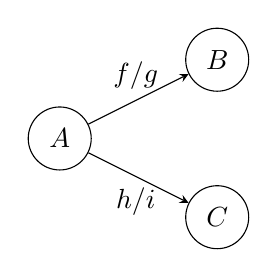
\begin{tikzpicture}[scale=1,-stealth]
\draw (0,-2) node[circle,fill=white,draw,minimum size = 8mm](A) {$A$};
\draw (2,-1) node[circle,fill=white,draw,minimum size = 8mm](B) {$B$};
\draw (2,-3) node[circle,fill=white,draw,minimum size = 8mm](C) {$C$};
\draw (A) --  node[left=1pt,above] {$f/g$} (B);
\draw (A) -- node[left=1pt,below] {$h/i$} (C);
\end{tikzpicture}
\caption{A statechart that may display unwanted non-deterministic behavior}
\label{fig:nsc}
\end{figure}
\newpar
This problem can be avoided by explicitly stating which transition should be prioritized. This is generally done by having all transition events be disjunct. \ref{fig:dsc} shows how this may be applied to the state chart from \ref{fig:nsc}. If both $f$ and $h$ are encountered at the same time, the chart now knows to always prioritize the transition to $B$, while transition to $C$ only happens if $h$ is present while $f$ is not.
\begin{figure}[h!]
\centering
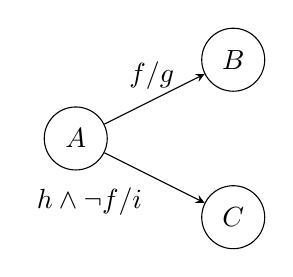
\begin{tikzpicture}[scale=1,-stealth]
\draw (0,-2) node[circle,fill=white,draw,minimum size = 8mm](A) {$A$};
\draw (2,-1) node[circle,fill=white,draw,minimum size = 8mm](B) {$B$};
\draw (2,-3) node[circle,fill=white,draw,minimum size = 8mm](C) {$C$};
\draw (A) --  node[left=1pt,above] {$f/g$} (B);
\draw (A) -- node[left=1pt,below left] {$h \wedge \neg f/i$} (C);
\end{tikzpicture}
\label{fig:dsc}
\caption{A fix to the chart's nondeterminism}
\end{figure}
\newpar
The big advantage of state charts compared to regular state machines is that they allow \tbf{superstates}, where an entire state machine may be contained within a single state of a ``higher level'' machine.
\begin{figure}[h!]
\centering
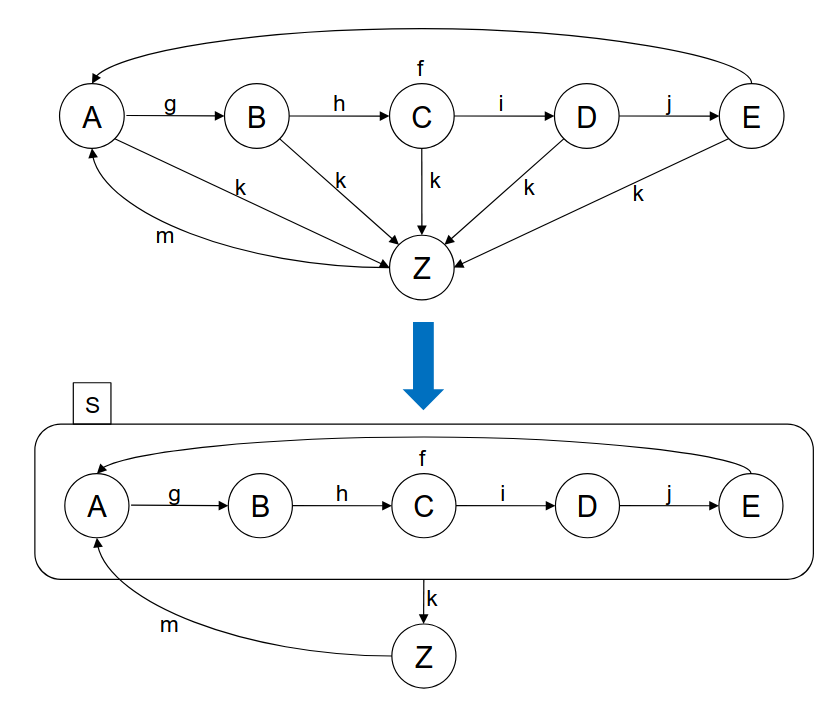
\includegraphics[scale=0.3]{figures/superstates}
\caption{Using superstates, this automaton can be drawn in a much tidier way.}
\label{fig:superstates}
\end{figure}
\newpar
As shown in \ref{fig:superstates}, this can make state charts significantly more readable than equivalent state machines. The basic type of superstate is the \tbf{OR-Superstate}, where an automaton may only be in one substate of a given superstate at any time. Later on, we will also introduce \tbf{AND-Superstates}, where an automaton is in \underline{all} of the substates of a given state at the same time.
\newpar
States within a state chart that don't contain substates are known as \tbf{basic states}. The set of superstates containing a given state are called the \tbf{ancestor states} of that state. When a basic state is active, all of its ancestor states are also considered active. If an active basic state and its ancestor state would both undergo a transition at the same time, the ``higher level'' transition of the ancestor state takes priority. See \ref{fig:priorities} for an example.
\begin{figure}[h!]
\centering
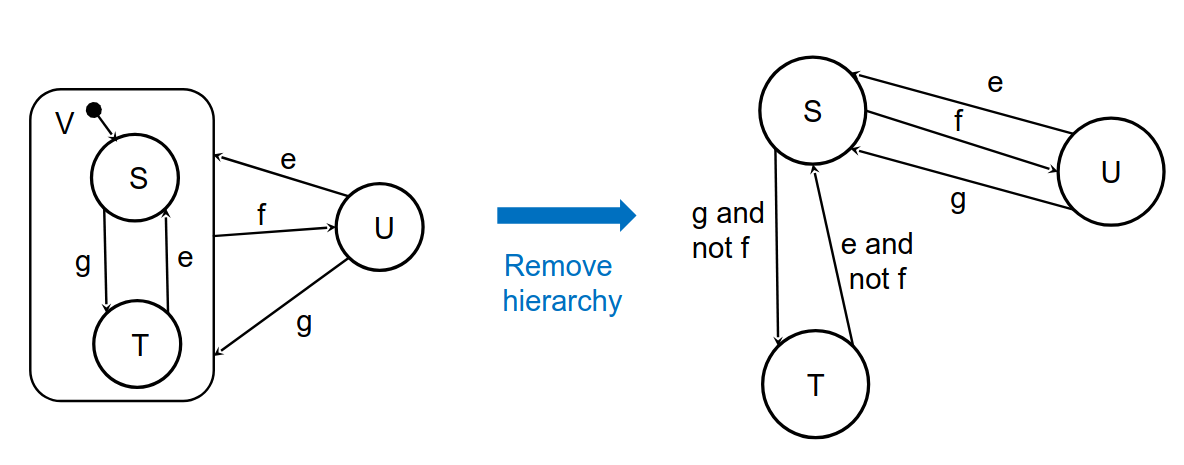
\includegraphics[scale=0.3]{figures/statechartpriorities}
\caption{A state chart using OR-Superstates and an equivalent state chart without hierarchy}
\label{fig:priorities}
\end{figure}
\newpar
By default, each automaton within a superstate contains a default starting state, and whenever the superstate is left, the automaton ``forgets'' what state it was in at that point and simply enters the starting state again if the ancestor state becomes active. This can be changed using \tbf{History States}.
\begin{figure}[h!]
\centering
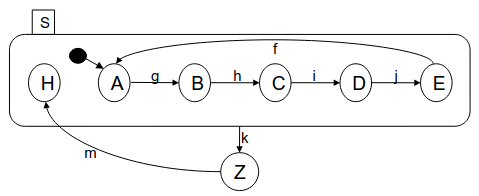
\includegraphics[scale=0.8]{figures/history}
\caption{A state chart that uses history states}
\label{fig:history}
\end{figure}
\newpar
In \ref{fig:history}, the state $H$ is the history state (the notation for history states seems frustratingly opaque and inconsistent - it seems like in most state charts, history states really aren't drawn in a special way, instead the historyness is only shown through them being called $H$.) This means that, whenever $H$ is entered, the subautomaton that $H$ is a part of instead enters the state it was in when it was last active. If the state has never been active, it enters the starting state $A$, signified here through an arrow and a black circle. If the state chart uses a \tbf{Deep History Mechanism}, that includes remembering what substates were last active, if the state the history state is pointing to is not a basic state.
%
\subsection{Petri Nets}
This section has been significantly shortened because of time pressure and general sleepyness, and also because the lecture spends ages on the trivial parts while completely rushing through the harder parts =w=
\newpage
A \tbf{place/transition net}, or petri net, is a tuple $N = (P, T, F, M_0$, such that:
\begin{itemize}
 \item $P$ is a set of \textit{places} (equivalent to an automatons states)
 \item $T$ is a set of \textit{events} (transition conditions)
 \item $F$ is a set called the \textit{flow relation}, connecting each place to an arbitrary amount of events and each event to an arbitrary amount of places using directional edges
 \item $K: P \to (\mathbb{N}_1 \cup \omega)$ assigns a capacity to each place (assumed to be $\omega$ if not explicitly stated)
 \item $W: F \to (\mathbb{N}_1)$ assigns a weight (= capacity) to each edge (assumed to be $1$ if not explicitly stated)
 \item $M_0: P \to \mathbb{N}_0$ is the initial marking, which specifies the amount of tokens each place starts with.
\end{itemize}
\newpar
A \tbf{condition/event net} is a petri net such that:
\begin{itemize}
 \item the net is \tbf{simple}, meaning that there can't be two seperate events directly connecting two places while going in the same direction (cycles are allowed)
 \item the net has no isolated elements
 \item the set of markings is closed with regards to firing and inverse firing (i.e. any marking can be turned into any other marking by the right sequence of firing and inverse firing)
 \item the net is \tbf{deadlock-free}, meaning that each reachable marking $M$ has at least one event $e$ that can be fired from $M$. This condition is also known as \tbf{weak liveness}.
 \item every place has a capacity of $1$ and intuitively represents a boolean condition.
\end{itemize}
A C/E net is called \tbf{cyclic} if any two markings are reachable from each other. C/E fulfills \tbf{liveness} if for each Marking $M$ and event $e$ there exists a Marking $M'$ reachable from $M$ that can fire $e$. A live petri net is always deadlock-free.
\newpar
A petri net can be specified by a matrix $M$ where the rows represent places and the columns represent events, with the value of each entry corresponding to the amount of tokes moved to (positive value) or from (negative value) the corresponding place by the corresponding transition. A petri net is called \tbf{contact-free} if capacities of places never prevent firing of the net. A petri net is called \tbf{pure} if it doesn't contain any self-loops.
%
\section{VHDL}
VHDL is a \tbf{Hardware Description Language}, meaning that it describes digital circuits (instead of abstract algorithms).
\newpar
VHDL code is split into \tbf{entities} and \tbf{architectures}. Entities describe ports, such as inputs (\textit{in}), outputs (\textit{out}), bi-directional ports (\textit{inout}), and \textit{buffers} (Output that the entity itself can read). An architecture defines the actual implementation of an entity - internal wiring, connection of signals, and assignment of values. For example, an OR gate could be implemented as:
\begin{verbatim}
entity orGate is
    port(a,b: in bit;
    c: out bit);
end orGate;
architecture arch1 of orGate is
begin
    c <= a or b;
end arch1;
\end{verbatim}
or:
\begin{verbatim}
entity orGate is
    port(a,b: in bit;
    c: out bit);
end orGate;
architecture arch2 of orGate is
begin
    c <= 1 when (a = '1' or b = '1') else 0;
end arch2;
\end{verbatim}
\newpar
There may be several architectures for a single entity. By default, the most recently analyzed architecture is the one that ends up being used.
\subsection{Testbenches}
A testbench is a VHDL Design without inputs or outputs, designed to test another VHDL Design, generally through Port mapping and verifying that the entity produces the correct outputs for given inputs. For example, a test bench for our OR gate could be realized as:
\begin{verbatim}
entity testbench is
 --empty
end testbench;

architecture test of testbench is
 signal d,e,f: bit := '0'

begin
 or1: entity orGate port map (a=>d,b=>e,c=>f);
 d <= not d after 10 ns;
end;
\end{verbatim}
The \tbf{port map} maps the signals $d,e,f$ in the software to the ports $a,b,c$ in the hardware. It is also possible to use positional association instead of explicit association, which means simply writing
\begin{verbatim}
architecture test of testbench is
 signal d,e,f: bit := '0'

begin
 or1: entity orGate port map (d,e,f);
 d <= not d after 10 ns;
end;
\end{verbatim}
after which the compiler will assign the ports based on the order of the signals in the port map. It is however good practice to always use explicit association.
\newpar
There are three concepts used in  testing:
\begin{itemize}
 \item \texttt{report}, for print-like outputs
 \item \texttt{assert}, for specifying conditions
 \item \texttt{severity}, for specifying how the statement should affect the run of a simulation
\end{itemize}
If needed, combinations of the three can be used within a single line:
\begin{verbatim}
report <message_string>
report <message_string> severity <severity_level>;

assert <condition>;
assert <condition> severity <severity_level>;
assert <condition> report <message_string>;
assert <condition> report <message_string> severity <severity_level>;
\end{verbatim}
If all three are used, the following happens: If the assertion is violated, the program sends a message \texttt{"message"}, and the whole thing is treated as an 'incident' with a predefined \texttt{severity\_level}. If an \texttt{assert} doesn't have a \texttt{severity\_level}, then the severity level will be \texttt{error}. If no \texttt{message\_string} is specified, the message will be \texttt{"Assertion Violation"}.
 If a \texttt{report} without an assertion does not have a \texttt{severity\_level}, the severity level is implicitly defined to be \texttt{note}.
 \newpar
 \texttt{report} statements are inherently sequential, meaning they can occur inside processes, but not (by themselves) in architectures. However, \texttt{assert}ions can be either sequential or concurrent.


\subsection{A Full Adder in VHDL}
\begin{verbatim}
entity fullAdder is

 port(a,b,cin: in bit;
      sum,cout: out bit);

end fullAdder;
\end{verbatim}
Dataflow description of the architecture:
\begin{verbatim}
architecture dataflow of fullAdder is

begin
 sum <= (a xor b) xor cin;
 cout <= (a and b) or (a and cin) or (b and cin);
end dataflow;
\end{verbatim}
\newpar
\tbf{Components} are entities used within a \tbf{structural definition} of an architecture, where a new architecture is defined as an interconnected circuit of already known smaller components. They are defined either via component and signal binding or via entity instantiation. For example, a fully structural definition of a full adder would be something like:
\begin{verbatim}
entity FULLADDER is
  port (A,B, CARRY_IN : in bit;
        SUM, CARRY    : out bit);
end FULLADDER;
 
architecture STRUCT of FULLADDER is
  component HALFADDER
    port (A, B       : in  bit;
          SUM, CARRY : out bit);
  end component;
 
  component ORGATE
    port (A, B : in  bit;
          RES  : out bit);
  end component;
  signal W_SUM, W_CARRY1, W_CARRY2 : bit;
 
begin
 
  MODULE1 : HALFADDER
    port map(A, B, W_SUM, W_CARRY1);
 
  MODULE2 : HALFADDER
    port map (W_SUM, CARRY_IN,
              SUM, W_CARRY2);
 
  MODULE3 : ORGATE
    port map (W_CARRY2, W_CARRY1, CARRY);
 
end STRUCT;
\end{verbatim}
\subsection{Data Types in VHDL}
\subsubsection{Standard data types}
The standard data types provided by VHDL are:
\newpar
\begin{tabular}{|c|c|}
    \hline
    bit & 0,1\\\hline
    boolean & true,false\\\hline
    character & most ASCII characters\\\hline
    integer & $-2^{31} - 1, \ldots, 2^{31}-1$\\\hline
    real & $-1.7e38, \ldots, 1.7e48$\\\hline
    time & 1fs, \ldots, 1hr\\\hline
\end{tabular}
\newpar
Users can also define their own datatypes, either as integer types:
\begin{verbatim}
 --64 bits
type small is range 0 to 63;

 --32 bits
type result32 is range 31 downto 0;

 --16 bits
subtype result16 is result32 range 15 downto 0;
\end{verbatim}
or as enumeration types:
\begin{verbatim}
type state is (idle,start,stop);
type hexDigits is (’0’, {…} , ’9’, ’A’, ’B’, ’C’, ’D’, ’E’, ’F’)
\end{verbatim}
\newpar
It is important not to get confused between statements like the following:
\begin{itemize}
 \item \texttt{signal S : integer range 0 to 3;}, meaning a number between 0 and 3
 \item \texttt{signal S : unsigned(3 downto 0);}, meaning an unsigned 3-bit integer (i.e. a number between 0 and 7)
\end{itemize}
Also note that for most datatypes, \texttt{downto} corresponds to little endian (i.e. most significant bit first), while \texttt{to} corresponds to big endian.

\subsubsection{std\_logic}
In realistic circuits, voltages may come in many forms not accurately described as simple boolean variables / bits. To model these, the datatype \texttt{std\_logic} is used, which contains signal types such as:
\newpar
\begin{tabular}{|c|c|}
    \hline
    0,1 & "Ground" and "High" Voltages\\\hline
    U & uninitialized\\\hline
    X & unknown, impossible to determine (generally a short circuit)\\\hline
    Z & high impedance (circuit connected to neither ground nor voltage)\\\hline
    H & weak drive, logic one (i.e. voltage behind resistor)\\\hline
    L & weak drive, logic zero\\\hline
    W & weak drive, undefined logic value\\\hline 
    - & don't care\\\hline
\end{tabular}
\newpar
These values take priority over each other in the following order: $X > (0 \sim 1) > W > (L \sim H) > Z$.
\newpar
\subsubsection{Arrays and Vectors}
\begin{verbatim}
type intArray is array (15 downto 0) of integer;
type bitArray is array (0 to 7) of bit;
type myMatrix is array (1 to 3, 1 to 3) of std_logic;
subtype myVector4 is std_logic_vector(3 downto 0);
\end{verbatim}
\subsection{Operators}
\newpar
\begin{tabular}{|c|c|c|}
\hline
    No. & Type & Examples\\\hline
    7 & Other Operators & \texttt{abs, not \textrm{(Negation of bits)}, ** \textrm{(exponentiation)}}\\\hline
    6 & Multipliying Operators & \texttt{*, /, mod, rem  \textrm{(remainder)}}\\\hline
    5 & Unary Operators & + (identity), - (negation of a numeric type)\\\hline
    4 & Addition Operators & \texttt{+, -, \&} (vector concatenation)\\\hline
    3 & Shift Operators &\texttt{sll, srl, sla, sra, rol, ror}\footnote[1]{}\\\hline
    2 & Relational Operators & \texttt{=, /= \textrm{(not equal)}, <, <=, >, >=}\\\hline
    1 & Logical Operators &\texttt{and, or, nand, nor, xor, xnor}\\\hline
\end{tabular}
\newpar
$^1$ - Shift operators ending in "l" are "logical", meaning vacated bits are filled with 0. Shift operators ending in "a" are "arithmetical", meaning vacated bits are filled with the value of the rightmost/leftmost bit. The operators "rol" and "ror" rotate the bits instead of shifting them.
\newpar
Operators with higher numbers in this table take priority over operators with lower numbers.
\subsection{Constants and Signals}
Constants work as expected in a programming language:
\begin{verbatim}
constant PI: real := 3.1415;
contant PERIOD: time := 100ns;
type vecType is array (0 to 3) of integer;
contant VEC: vecType := (2,4,-1,7)
\end{verbatim}
Signals represent a wire or register. They can be of any data type, can be declared in architectures only.
\begin{verbatim}
signal sum: std_logic;
signal clk: bit;
signal data: std_logic_vector(0 to 7) := "00X0X011";
signal value: integer range 16 to 31 := 17;
\end{verbatim}
Signals assignments are performed \tbf{concurrently}, meaning that they are sequentially collected until the process is stopped, and then collectively performed in parallel after al processes are stopped.
\newpar
Signals can be assigned with either an explicit user-defined time delay ("after 10ns", etc.), or with an implicit small delta delay:
\begin{verbatim}
sum <= (a xor b) after 2 ns; -- explicit delay
data(1) <= 'x'; -- implicit delay
\end{verbatim}
Signal assignments can also include conditionals. This can be done using the when-else condition:
\begin{verbatim}
clk <= '0' after 5ns when clk = '1' else '1' after 7ns when clk = '0';
a <= "1000" when b = "00" 
else "0100" when b = "01" 
else "0010" when b= "10" 
else "0001" when b = "11";
\end{verbatim}
Or using the with-select condition:
\begin{verbatim}
with b select a <=
	"1000" when "00",
	"0100" when "01",
	"0010" when "10",
	"0001" when "11";
\end{verbatim}
Neither of the two conditionals may be used inside a process. Within the finished hardware, conditions like this are realized using a multiplexer. Custom multiplexer code would look something like this:
\begin{verbatim}
entity mux is
port (i3, i2, i1, i0: in bit;
    sel: in bit_vector(1 downto 0);
    otp: out bit);
end;    

architecture wSelect of mux is
begin
    with sel select
    otp <= i0 when "00",
    i1 when "01",
    i2 when "10",
    i3 when others;
end;
\end{verbatim}
\subsection{Variables}
Variables work like variables in other programming languages. They store temporary values and are only usable in processes, procedures and functions. \tbf{Usage of them is not recommended in VHDL for synthesis.} Unlike signal assignments, variables assignments are performed sequentially as they are encountered in the code.
\subsection{Processes}
We've already seen two styles of modelling using VHDL: A Dataflow architecture uses concurrent signal assignment statements, while a structural architecture uses only component instantiation statements. We will now learn a third style: \tbf{Behavioural architecture}, which uses  \tbf{process statements}. A process is simply a set of statements that are executed sequentially-ish:
\begin{verbatim}
signal clk : std_logic := '0';
clk_gen: process ( )
begin
 clk <= ‘0’;
 wait for 10 ns;
 clk <= ‘1’;
 wait for 10 ns;
end process;
\end{verbatim}
VHDL supports four different types of wait statements:
\begin{itemize}
    \item \texttt{wait on} waits until one of the given signals changes (e.g. \texttt{wait on a,b,c;}).
    \item \texttt{wait until} waits until the given condition is met (e.g. \texttt{wait until (clkEvent and clk = '1')}).
    \item \texttt{wait for} waits for a specified amount of time (e.g. \texttt{wait for 25 ns;}).
    \item \texttt{wait} waits indefinitely.
\end{itemize}
Only simple signal assignments are allowed inside a process. When a simulation starts, each process will be executed at least once. Afterwards, they will loop infinitely. If the process has a \textit{sensitivity list}, a new iteration will occur whenever a signal from the sensitivity list changes:
\begin{verbatim}
entity DFF is
port (D, clk: in std_logic;
Q: out std_logic);
end DFF;
architecture rtl of DFF is
begin
 p : process(clk) -- sensitivity list
 begin
 if (clk‘event) and (clk=`1`) then
  Q <= D;
 end if;
 end process p;
end rtl;    
\end{verbatim}
Processes with sensitivity lists are equivalent to processes without a sensitivity loop that have \texttt{wait on} statements instead:
\begin{verbatim}
entity DFF is
port (D, clk: in std_logic;
Q: out std_logic);
end DFF;
architecture rtl of DFF is
begin
 p : process
 begin
  if (clk‘event) and (clk=`1`) then
   Q <= D;
  end if;
  wait on clk; -- equivalent wait statement
 end process p;
end rtl;
\end{verbatim}
Processes are not allowed to have subprocesses. They always loop, and are often used to specify sequential hardware. Everything in VHDL is implicitly part of a "main" process.
\subsection{Statements}
\texttt{if}-Statements and \texttt{case}-Statements are comparable to \texttt{if}-Statements and \texttt{switch}-statements in other languages. Both of them can be nested. Conditions in \texttt{if}-Statements can be any boolean expression.
\begin{multicols}{2}
\begin{verbatim}
if a = b then
…
elsif a > b or a > c then
…
else
…
end if;    
\end{verbatim}
\begin{verbatim}
case a is
when "01" =>
…
when "10" =>
…
when others =>
null
end case;    
\end{verbatim}
\end{multicols}
\newpar
As seen here, a case where nothing happens can be specified using the \texttt{null} Statement.
\newpar
VHDL also supports \texttt{loop}s. Here are two variants of a clock that counts up to 10, incrementing once every 5ns, using a \texttt{while} loop and a \texttt{for} loop:
\begin{multicols}{2}
\begin{verbatim}
constant MAX_SIM_TIME : time := 50 ns;
constant PERIOD : time := 10 ns;
...
clk_gen: process (clk)
begin
 while NOW < MAX_SIM_TIME loop --!
  clk <= not clk ;
  wait for PERIOD/2;
 end loop;
 wait;
end process clk_gen;
\end{verbatim}
\begin{verbatim}
constant MAX_CYCLES : integer := 10;
constant PERIOD : time := 10 ns;
...
clk_gen: process (clk)
variable cnt: integer := 0
begin
 for cnt in 1 to MAX_CYCLES loop --!
  clk <= not clk ;
  wait for PERIOD/2;
 end loop;
 wait;
end process clk_gen;
\end{verbatim}
\end{multicols}
\newpar
And a third variant using the \texttt{exit when}-Statement:
\begin{verbatim}
constant MAX_CYCLES : integer := 10;
...
clk_gen: process (clk)
variable cnt: integer := 0;
begin
 L1: loop
  clk <= not clk;
  cnt := cnt + 1;
  wait for 5ns;
 exit when cnt > 2*MAX_CYCLES; --!
end loop;
wait;
end process clk_gen;
\end{verbatim}
\newpar
During synthesis, all loops have to be unrolled, meaning that loops with a non-static range are non-synthesisable. It is generally good practice to only use loops in testbenches.
\subsection{Functions and procedures}
Apart from entities and architectures, VHDL also supports functions and procedures, similar to traditional programming languages. A \tbf{Function} has a return value and can be used in statements:
\begin{verbatim}
architecture rtl of example is
 signal test : integer := 0;
 ...

begin
 function b2i(b : bit) return integer is
 begin
  if b = '1' then
   return 1;
  else
   return 0;
  end if;
 end b2i;

 test <= b2i(’0’);
end;
\end{verbatim}
Functions can be overloaded, meaning that there can be Functions with the same name but different type signatures. By default, functions have to be \tbf{pure}, meaning they are free of side effects - formally $f(a)$ always returns the same value if $a$ is the same. An impure function can be declared by prepending the function with \texttt{impure}. This will let the function gain access to all variables and signals outside of its scope.
\newpar
A \tbf{Procedure} can be seen as a function without a return value. Instead, it has \texttt{in, out} or \texttt{inout}-signals, similar to an entity:
\begin{verbatim}
architecture behave of ex_procedure_simple is
 signal r_TEST : std_logic_vector(7 downto 0) := X"42";

-- Purpose: Increments a std_logic_vector by 1
 procedure INCREMENT_SLV (
  signal r_IN : in std_logic_vector(7 downto 0);
  signal r_OUT : out std_logic_vector(7 downto 0)
  ) is
  begin
   r_OUT <= std_logic_vector(unsigned(r_IN) + 1);
  end INCREMENT_SLV;
...
 signal test : std_logic_vector(7 downto 0) := (others => '0');
...
 test_p: process
 begin
  INCREMENT_SLV(test, test);
 end test_p;
\end{verbatim}
Because Procedures do not return anything, they can't be used in statements. They can still be used inside of processes, or, if \texttt{out} and \texttt{inout} parameters are signals, as their own processes.
\subsection{Synthesisable vs Non-Synthesisable Code}
Only a subset of VHDL statements is \tbf{synthesisable} (i.e. compilable with the output being hardware). Non-synthesisable statements include time statements, asserts, and dynamic loops.
\newpar
You can work around many of these restrictions. For example, the following code is non-synthesisable, because it uses a \texttt{wait}-Statement:
\begin{verbatim}
architecture behavior of testbench is
begin
 enable <= '0';
 wait for 100 ns; -- !
 enable <= '1'
end behavior;
\end{verbatim}
However, the following code is synthesisable:
\begin{verbatim}
architecture behavior of realCircuit is
signal cnt : unsigned(3 downto 0) := (others => '0');
begin
 process ( clk )
 begin
  if rising_edge( clk ) then
   if cnt < 10 then -- assume clk  period is 10 ns
    cnt <= cnt + 1;
    enable <= '0';
   else
    cnt <= (others => '0');
    enable <= '1';
   end if;
  end if;
 end process;
end behavior;
\end{verbatim}
\newpar
Many statements in VHDL are technically synthesisable, but are best avoided, generally because they quickly lead to significant, often unexpected, increases in hardware complexity. These include:
\begin{itemize}
 \item division or multiplication with numbers that aren't powers of 2
 \item \texttt{if rising\_edge (clk)} with \texttt{else}
 \item latches
\end{itemize}
\newpar
a \tbf{latch} is a memory element that is triggered by a changes immediately whenever the input changes:
\begin{verbatim}
architecture rtl of latch is
…
begin
 process (E, D) begin
  if E = ’1’ then
   Q <= D;
  end if;
 end process;
end;
\end{verbatim}
The big problem with latches is that they leaf to uncertainty in a circuit's timing behavior. You can avoid latches by including a clock and triggering things only on rising edges, and by stating all possibilities in if statements.
\subsection{Simulation}
A simulation works in the following way:
\begin{itemize}
\item Initialization:
\begin{itemize}
 \item Initialize all signals
 \item Set simulation time to 0
 \item Execute all processes once
 \item Start simulaton cycles
\end{itemize}
\item Simulation cycles:
\begin{itemize}
 \item update signals
 \item execute processes
 \item repeat
\end{itemize}
\item Simulation ends when:
\begin{itemize}
 \item No more signal changes are possible
 \item A maximum simlulation time has been reached
 \item An explicit \texttt{wait} is encountered
\end{itemize}
\end{itemize}
\newpar
Values are assigned to signals using a \tbf{transaction list}. The list contains entries of the form $(s,v,t)$, meaning ``signal $s$ is set to value $v$ at time $t$''. Processes are similarly reactivated using a \tbf{process activation list}, with entries of the form $(p,t)$ (``process $p$ resumes at time $t$'').
\subsection{Delay Modeling}
Real components always work on a delay. \tbf{Delay of components} can be modeled in VHDL using the \texttt{inertial} Keyword:
\begin{verbatim}
output <= not input after 10 ns;
-- with inertial delay:
output <= reject 5 ns inertial not input after 10 ns;
\end{verbatim}
If a signal assignment happens for an amount of time shorter than the signals inertial delay, then the signal doesn't change at all.
\newpar
There is also the Keyword \texttt{transport} to model the \tbf{delay of wires}:
\begin{verbatim}
output <= not input after 10 ns;
-- with transport delay:
output <= transport not input after 10 ns;
\end{verbatim}
A signal that uses \texttt{transport} delay always gets changed after the specified time.
%
\chapter{Design Space Evaluation}
Design Space Evaluation is the process of considering different possible ways to realize a given plan and comparing them based on criteria such as:
\begin{multicols}{2}
\begin{itemize}
 \item Cost
 \item Performance
 \item Power consumption
 \item Quality
\end{itemize}
\end{multicols}
\newpar
'Cost' can be further split into factors such as:
\begin{multicols}{2}
 \begin{itemize}
  \item Manufacturing cost
  \item Design cost
  \item Field support
  \item Administration
  \item Design time
  \item[\vspace{\fill}]
 \end{itemize}
\end{multicols}
While 'Performance' comes down to factors like:
\begin{multicols}{2}
\begin{itemize}
 \item Clock Frequency / Operations per Second
 \item Bandwidth
 \item Quality of service
 \item[\vspace{\fill}]
\end{itemize}
\end{multicols}
\newpar
Note that especially in safety-critical systems, it is preferable to accept a worse average runtime if it leads to a better worst case runtime and more predictability. For example, caching is usually avoided because of its inherent unpredictability.
\newpar
Within the context of Embedded Systems, common decision points include choosing between:
\begin{multicols}{3}
\begin{itemize}
 \item ASICs (Application specific integrated circuits)
 \item Field Programmable Gate Arrays (FPGAs)
 \item Microprocessors
 \item Microcontrollers
 \item Different Memory Architectures
 \item Different Interfaces (I$^2$C, SPI, CAN, \ldots)
 \item Different possible Sensors \& Actuators
 \item Different possible AD and DA converters
 \item etc.
\end{itemize}
\end{multicols}
\newpar
Formally, this comes down to a \tbf{multiobjective optimisation problem}.
\section{Power Consumption}
Generally, \tbf{power} is the most important constraint in Embedded Systems, and thus minimizing power consumption is one of the primary concerns during the design process. Modern processors have a power density of up to $100 \frac{W}{cm^2}$!
\newpar
Minimizing the power consumption leads to less pressure for the power supply and for voltage regulators and a much lower risk of overheating (also meaning less effort needed to introduce cooling). Naturally it also means lower costs.
\newpar
Low power design techniques include the usage of different components such as \tbf{low-power transistors}, which tend to come with drawbacks in speed. It may also involve dynamic power management, i.e. sleep modes (temporarily switching off components that aren't needed). Switching off the clock of a flip-flop specifically is known as \tbf{clock gating}. Dynamic power management naturally brings with it the cost of requiring additional logic. One can also use \tbf{dynamic voltage and frequency scaling}, where the power supply voltage is lowered when needed and the clock frequency is lowered accordingly.
\newpar
The power consumption $P$ of a CMOS circuit is
\begin{equation*}
P = \alpha C_L V_{DD}^2f
\end{equation*}
Where:
\begin{itemize}
 \item $\alpha$ is the \textit{switching activity} or \textit{activity factor}, defined as the probablity that a circuit node changes from logic 0 to logic 1 in any given clock cycle,
 \item $C_L$ is the \textit{load capacitance}, i.e. the capacitance between the output of a circuit and ground,
 \item $V_{DD}$ is the supply voltage,
 \item and $f$ is the clock frequency.
\end{itemize}
\newpar
For a more detailed breakdown of this equation, I found \href{https://cdn.intechopen.com/pdfs/82415.pdf}{\textit{Power Consumption in CMOS
Circuits} by Len Luet Ng et al.} to be helpful.
\newpar
The delay of a CMOS circuit is
\begin{equation*}
\tau = k \cdot C_L \frac{V_{DD}}{(V_{DD}-V_t)^2}
\end{equation*}
Where $k$ is a contant that depends on the circuit and $V_t$ is the threshold voltage, i.e. the voltage defined as the cutoff between a logical ``1'' and a logical ``0''.
\newpar
The important takeaway from these equations is that
\begin{equation*}
P \propto V_{DD}^2, \text{ while } \tau \propto \frac{1}{V_{DD} + \frac{1}{V_{DD}}}.
\end{equation*}
This means that, by decreasing the supply voltage of a circuit, the circuit's power consumption can be decreased quadratically, while the circuit's delay increases roughly linearly (by a pretty generous definition of ``roughly'').
%
\section{Quality Testing}
All manufacturing processes are inherently prone to defects. Naturally, defective parts should not be delivered to customers. Therefore, a need arises for \tbf{test processes} to distinguish good components from faulty ones. Testing can incur significant costs (the slides state an unsourced figure of ``up to 60\%''). Naturally, these still cannot identify 100\% of defective parts. There are many different approaches of testing for different types of components and the systems they make up. Parts are also susceptible to aging, which leads to parts which were previously defect-free to become defective over time. Lastly, parts may be susceptible to external effects like changing temperatures, noise or radiation.
\newpar
The fraction of defective delivered parts over total delivered parts is known as the \tbf{Defect Level (DL)} or as the number of \tbf{test escapes}. Naturally, a high defect level can lead to a loss of reputation and eventually to legal penalties. The fraction of defective-free part over all parts is known as the \tbf{Yield}. A higher lead naturally leads to lower testing costs and fewer test escapes. Finally, as already defined in the introduction, \tbf{Reliability} measures the probability that a part will work correctly over a given time, and is incredibly important especially for safety-critical systems. Ideally, a system should be able to undergo \tbf{graceful degradation}, meaning that as the system degrades, performance merely decreases gradually instead of suddenly catastrophically failing.
\newpar
Generally, a specification will include required bounds on quality parameters. For example, the IEC 61508 standard defines four safety integrity levels (SIL 1 through SIL 4). By this definition, an SIL 1 system must have a failure probability per hour lower than $\frac{1}{10^5}$, while an SIL 4 system needs to meet a much stricter requirement of at most $\frac{1}{10^8}$ failures per hour.
%
\section{Pareto Frontier}
A solution of the multiobjective optimisation problem posed by design space exploration is given by a vector $V = (v_1, \hdots, v_n)$ of parameters describing the performance, costs etc. associated with a possible realisation of a specification. We define these parameters in such a way that higher values are always better, which means that, for parameters describing a cost, we need to either take the negative or the inverse of the cost value. Naturally, these parameters are generally only estimates, since determining the exact values would have to involve production of every single possible solution at a non-trivial scale.
\newpar
A natural way of discarding inferior solutions is given by \tbf{pareto superiority}. We say that a solution $A$ is pareto-superior to a solution $B$ iff we have both $\forall j(a_j \geq b_j)$ ($A$ is at least as good as $B$ in every aspect) and $\exists i(a_i > a_j)$ (There is at least one aspect of $A$ that is better than $B$). It should be intuitively obvious that if $A$ is superior to $B$ in every single criterium considered, then $A$ is preferable over $B$. The set of all solutions not dominated by any other solution is known as the \tbf{Pareto Frontier}.
%
\chapter{Hardware}
\thispagestyle{fancy}
\section{Microprocessors vs Microcontrollers}
A Microprocessor consists of \tbf{only a computing unit}, which then needs to be complemented by memory, I/O interfaces etc. Microprocessors are fast, but often  expensive.
\newpar
Meanwhile, a Microcontroller is a \tbf{System-on-chip (SOC)}. It already contains memory, timers, voltage converters, and at least one I/O interface (generally even multiple). They are slower than microprocessors, but are cheap and energy efficient.
%
\section{Memory}
Technological improvements to computer memory size and access times are currently made at a much slower pace than improvements to processor cycle times. This \tbf{Memory Wall} is a key challenge in the development of new AI models and, more generally, in most high performance computing applications.
\begin{figure}[h!]
 \centering
 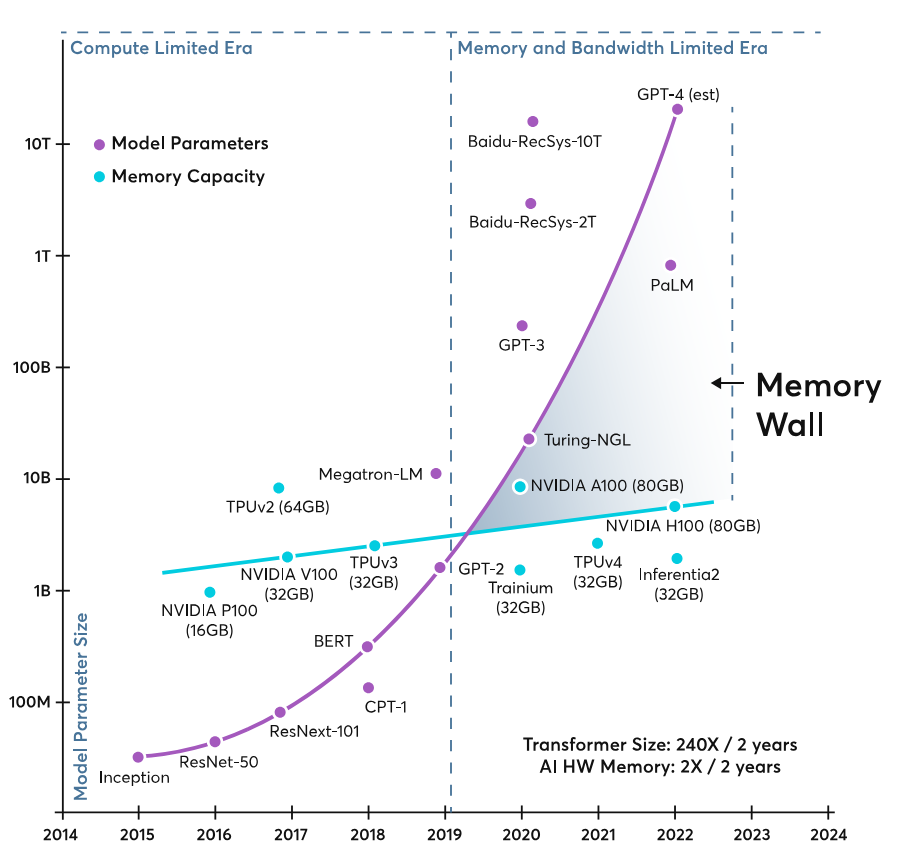
\includegraphics[scale=0.3]{figures/memorywall.png}
 \caption{The memory wall in action (Source: \href{https://ayarlabs.com/wp-content/uploads/2024/05/Memory_Wall_Chart.svg}{ayarlabs})}
\end{figure}
\newpar
The \tbf{Principle of Locality} is the Observation that programs tend to use data with addresses near those they have already used recently. It can be further split into \tbf{Temporal Locality}, which means that recently referenced items are likely to be referenced again soon, and \tbf{Spatial Locality}, meaning that items with nearby addresses are often referenced around the same time. Modern memory architectures exploit these properties through \tbf{caching}, where several types of memory exist within a system, and items  are placed in faster memory or slower memory depending on how likely it is that they will be needed in the near future.
\newpar
The most basic types of memory, ordered by speed, are:
\begin{enumerate}
 \item Registers
 \item Cache, Scratchpad Memory (SPM)
 \item Main Memory (RAM)
 \item Secondary Storage (SSD, HDD)
\end{enumerate}
On its own, a processor tends to only include registers and cache or SPM. The registers of a processor could technically be considered a particularly fast type of cache. Fast caches have to be placed near the processing unit - the increases in signal travel time and especially in ambient noise that come with longer wires are actually relevant factors in determining memory speed.
%
\subsection{Cache Design}
Some key questions of cache design are:
\begin{itemize}
 \item Which memory blocks do we place into which cache blocks?
 \item How do we detect if and where a block is in the cache?
 \item Which cache block is replaced after a \tbf{cache miss}, i.e. when an item is needed that isn't in the cache yet?
 \item What happens if we write new things into memory?
 \item How do we deal with multi-core architectures?
\end{itemize}
A \tbf{direct mapping cache} is a cache where the adress of any item in cache is simply the item's adress in main memory modulo the number of cache blocks. A cache where any item can occupy any block is known as an \tbf{associative cache}. To use an associative cache, one needs to specify what happens when the cache is full - a predefined \tbf{cache replacement strategy} is needed. Common cache replacement strategies include:
\begin{itemize}
 \item FIFO (first in, first out)
 \item LRU (least recently used)
 \item random selection
\end{itemize}
Interestingly, random selection is provably optimal in cases where the order that items are needed in is provided by an \textit{oblivious adversary} (See lecture ``Algorithm Theory'' for more details). However, for real-time embedded systems, predictability is key, which means that non-deterministic cache algorithms are used. For a worst case execution time analysis, one has to assume that almost every access to the cache leads to a cache miss.
%
\subsection{Scratch Pad Memory}
A scratch pad memory architecture maps small physical memory addresses directly into the CPU's address space. Frequently used variables and instructions can thus be allocated to the scratch pad memory \tbf{at compile time}. This leads to \tbf{fast and predictable behavior and lower energy consumption}, especially compared to associative cache architectures. Some architectures contain both caches and SPM, leading to a hierachical memory structure:
\begin{figure}[h!]
\centering
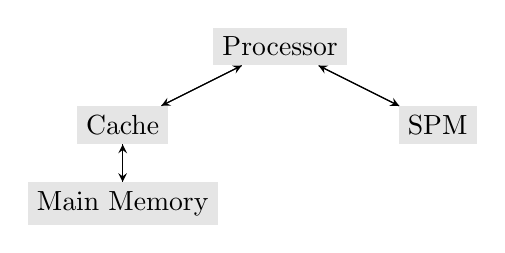
\begin{tikzpicture}[scale=1,-stealth]
\draw[fill=white!90!black] (0,0) node[fill](P) {Processor};

\draw[fill=white!90!black] (-2,-1) node[fill](C) {Cache};
\draw[fill=white!90!black] (-2,-2) node[fill](M) {Main Memory};

\draw[fill=white!90!black] (2,-1) node[fill](S) {SPM};

\draw (P) to (C);
\draw (C) to (P);
\draw (P) to (S);
\draw (S) to (P);
\draw (C) to (M);
\draw (M) to (C);

\end{tikzpicture}

\caption{A memory architecture that combines caching with SPM}
\label{fig:memoryhierarchy}
\end{figure}
%
\subsection{I/O Access}
The two most basic ways of handling I/O are \tbf{memory-mapped I/O}, where components get mapped directly into controller address space, and \tbf{port-mapped I/O}, also known as \tbf{programmed I/O}, where the CPU transfers bytes using a special instruction. However, both of those have the major disadvantage of keeping the CPU busy, with updates requiring polling.
\newpar
Most microprocessors and -controllers include a component that allows \tbf{DMA (Direct Memory Access)}. These are dedicated components that allow the CPU to do other work or sleep during a data transfer. However, the CPU still needs to initiate the transfer on its own. Typically, the CPU then receives an interrupt from the DMA once the transfer is done.
\newpar
Usage of DMAs brings with it the problem of \tbf{cache coherency}. Imagine the following scenario:
\begin{itemize}
 \item The CPU accesses location X in memory and stores the current value of X in cache
 \item Subsequent operations on X update the cached copy of X, not the external memory version of X (since updating the external version would mean dealing with slow memory speeds, defeating the whole purpose of a cache.)
 \item Whenever an outside device now tries to access X, that device will \tbf{recieve the old value of X.} Similary, if a device updates X in main memory, then \tbf{the CPU will be working with an outdated version of X.}
\end{itemize}
A simple cache consistency protocol consists of having both the CPU and outside devices broadcast an ``invalidate'' flag on every write to memory, signaling to each other that a value has become outdated. Alternatives include having a \tbf{write-through} or \tbf{write-around} cache instead of a write-back cache, meaning that everything that is written to cache is copied to main memory immediately. This sacrifices speed on writes (but still leaves the benefits caches have for reads).
%
\subsection{Interrupts}
Interrupts allow the CPU to be notified about important events. An interrupt generally gets processed as follows:
\begin{enumerate}
 \item an interrupt request is triggered
 \item the CPU stops its current exectution flow and saves its current state to memory
 \item the CPU executes the interrupt service routine associated with the specific interrupt request
 \item the CPU reloads its state and continues normal operation
\end{enumerate}
Modern CPUs feature at least one programmable interrupt controller (PIC) that manages interrups along several lines (to allow several devices to send interrupts) by assigning priorities and delaying or outright ignoring low-important interrupts.
%
\section{Communication}
In order to communicate with each other, digital devices need to send \tbf{modulated signals}. Signal modulation can be split into analog (i.e. continuous) methods and digital (i.e. discrete) methods.
\subsection{Pulse Width Modulation}
Pulse Width Modulation \tbf{(PWM)} is a digital modulation method that is very common in sensor and actuator interfaces. It represents a signal as a rectangular wave, where each rate corresponds to a certain linear speed at which the resulting analog symbol should change.
\begin{figure}[h!]
\centering
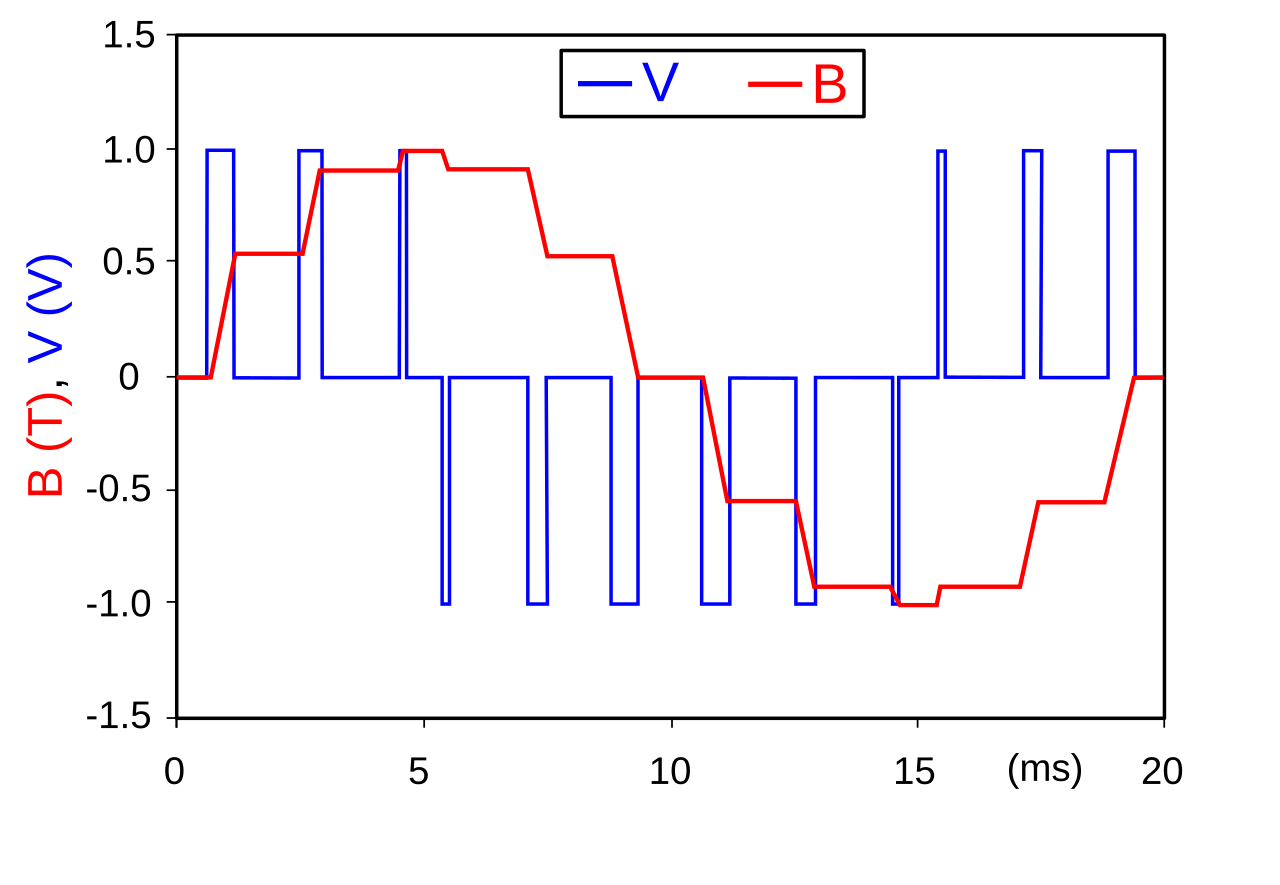
\includegraphics[scale=0.15]{figures/3StatePWM.png}
\caption{A digital signal representing a sine-like curve using 3-Level PWM. (Source: \href{https://en.wikipedia.org/wiki/File:PWM,_3-level.svg}{Wikipedia})}
\label{fig:3StatePWM}
\end{figure}
\begin{figure}[h!]
\centering
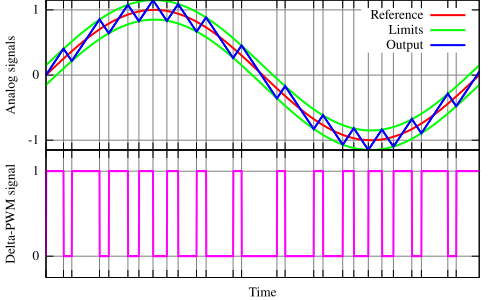
\includegraphics[scale=0.5]{figures/DeltaPWM.png}
\caption{A similar curve represented using 2-Level Delta PWM. (Source: \href{https://en.wikipedia.org/wiki/File:Delta_PWM.svg}{Wikipedia})}
\label{fig:DeltaPWM}
\end{figure}
\newpar
The \tbf{Duty Cycle D} of a 2-Level PWN Signal describes the proportion of ``on'' time during a given interval.
\newpar
The most common way of realizing 2-Level PWM is \tbf{intersective PWM}, where the PWM output is switched every time a sawtooth wave with the desired growth rate intersects with the input waveform. Another method is \tbf{Delta PWM}, where '0' level represents a negative slope and the output is switched every time the output signal exceeds a given upper or lower bound around the input signal (see \ref{fig:DeltaPWM}).
%
\subsection{Bus Standards}
A large number of different bus standards exist, all with their own capabilities, benefits and drawbacks. Protocols where data is transferred based on a common clock are called \tbf{synchronous}, while ones without a clock are called \tbf{asynchronous}. An example of an asynchronous protocol would be UART (universal asynchronous receiver-transmitter), which wasn't covered in detail by the lecture. The protocols covered by the lecture are:
\newpar
\tbf{I$^2$C}:
\begin{itemize}
 \item stands for ``inter-integrated circuit'', sometimes alternatively abbreviated to I2C or IIC
 \item main-sub architecture\footnote{
 Many places, including the original slides presented by Prof. Amft, still use the terminology ``master-slave''. Since many people, myself included, find this terminology inappropriate, I will be using ``main-sub'', which has established itself as a common alternative that still works with any relevant acronyms.}
 - a controller ('main') generates a clock signal an sends out requests for data, which are then replied to by the targets ('sub').
 \item one single data line (\texttt{SDA}) and clock line (\texttt{SCL}) shared by all connected devices
 \item slow and high-power but cheap
\end{itemize}
\begin{figure}[h!]
\centering
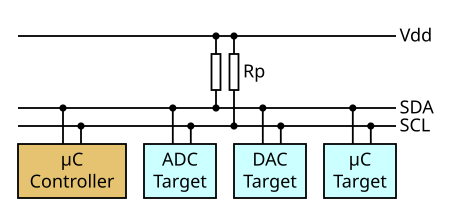
\includegraphics[scale=0.5]{figures/I2C.png}
\caption{The I2C bus architecture}
\label{fig:DeltaPWM}
\end{figure}
\tbf{SPI}:
\begin{itemize}
 \item main-sub architecture. unlike I2C, SPI only supports a single controller.
 \item two seperate data buses: \texttt{MOSI} (main out sub in) and \texttt{MISO} (main in sub out). This has the major advantage of allowing data to be transmitted and recieved simulataneously (making SPI a \tbf{full duplex protocol}).
 \item additional lines $\overline{\text{SS}}$ (sub select)
 \item fast and low-power at the cost of more required space and more complex logic
\end{itemize}
\begin{figure}[h!]
\centering
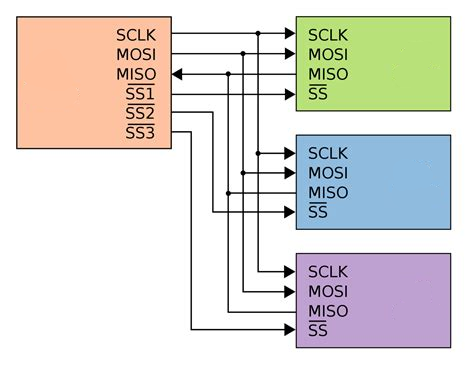
\includegraphics[scale=1.5]{figures/SPI.png}
\caption{The SPI bus architecture (controller on the left, targets on the right)}
\label{fig:DeltaPWM}
\end{figure}
\begin{figure}[h!]
\centering
\begin{tabular}[h!]{|c|cccccc|}
\hline
Name & synchronicity & main-sub? & full duplex? & speed & power & cost\\\hline
I2C & synchronous & yes & no & low & high & low\\
SPI & synchronous & yes & yes & high & medium & high\\
UART & asynchronous & no & yes & lowest & lowest & lowest\\
\hline
\end{tabular}
\caption{Comparison of common bus architectures}
\end{figure}
UART is often considered somewhat outdated and is being gradually replaced by more modern architectures like I2C, SPI, or USB.
%
\section{Debugging}
The general methods of debugging an embedded system, ordered by increasing realism and increasing effort, are:
\begin{enumerate}
 \item Emulation (Imitate behavior of the target without necessarily imitating the internal state of the target)
 \item Simulation (Evaluate with an accurate model of the target system)
 \item On-Targets (Evaluate on actual target hardware within a lab or simulation environment)
 \item On-Field (Evaluate on actual target hardware within in the targeted application environment)
\end{enumerate}
Testing can prove the presence of errors, but in order to prove the absence of errors, more complicated methods of Program and Hardware Verification are needed, which are not covered in this course.
%
\subsection{JTAG}
JTAG is a standard for testing and debugging integrated circuits, introduced in 1985. It introduces a \tbf{Test Access Port (TAP)} to integrated circuits, which allow easy access to internal logic of ICs and PCBs via connection of TAPs to an external testing device.
\newpar
JTAG specifies a serial protocol with four to five lines: TDI (Test Data In), TDO (Test Data Out), TCK (Test Clock), TMS (Test Mode Select), TRST (Test Reset, Optional). It has no maximum speed, but is typically used with a speed of 10-100 MHz.
\begin{figure}[h!]
\centering
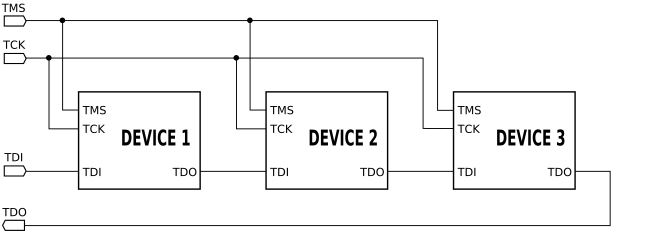
\includegraphics[scale=0.5]{figures/JTAG.png}
\caption{The structure of a daisychained JTAG interface. (Source: \href{https://en.wikipedia.org/wiki/File:Jtag_chain.svg}{Wikipedia})}
\label{fig:DeltaPWM}
\end{figure}
Using JTAG, one can recover ``dead'' boards where a microcontroller doesn't boot. No specific software needs to be installed on the target. The TAP controller itself implements a stateful protocol to access the test registers. JTAG is available on most modern embedded devices. It is also a common way of hacking devices such as video game consoles, if no sufficient encryption is present.
%
\section{Signal Processing}
Signals are differentiated by whether they are \tbf{time-continuous or time discrete} (i.e. whether a signal is always present or whether a set of seperate short pulses is sent with some delay inbetween) and by whether the possible amplitues of a signal are a limited set of discrete (digital) values or a continuous (analog) range ofvalues. ADC (Analog-Digital-Conversion) always includes discretization in both time and amplitude.
\subsection{Direct Conversion}
\begin{figure}[h!]
\centering
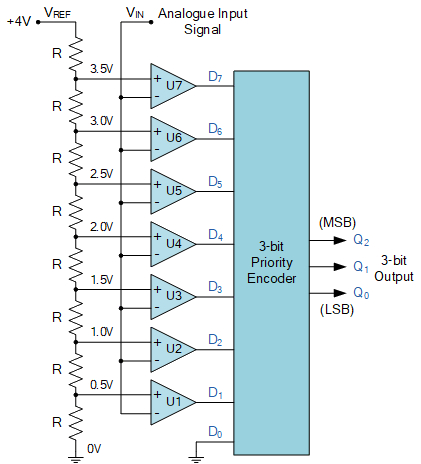
\includegraphics[scale=2]{figures/ADC}
\caption{A basic ADC (Source: \href{https://www.electronics-tutorials.ws/combination/analogue-to-digital-converter.html}{electronics-tutorials.ws})}
\label{fig:ADC}
\end{figure}
\ref{fig:ADC} shows a realization of a basic ADC that encodes an $n$-bit output using $2^n - 1$ comparators and $2^n$ resistors. A simple realization like this inherently allows for very high conversion frequencies ($> 1$GHz).
\begin{figure}[h!]
\centering
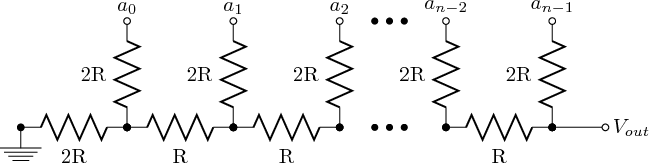
\includegraphics[scale=0.5]{figures/DAC}
\caption{A basic DAC (Source: \href{https://en.wikipedia.org/wiki/File:R2r-ladder.png}{Wikipedia}}
\label{fig:DAC}
\end{figure}
\newpar
\ref{fig:DAC} shows that a DAC can be realized in an even simpler way. The given resistor ladder  encodes an $n$-bit input using $2n$ resistors. $a_0$ represents the least significant bit while $a_{n-1}$ represents the most significant bit.
\newpar
Basic ADC or DAC designs like the ones just presented have the disadvantage of requiring the resistances of all of the present resistors to be sufficiently accurate.
\subsection{Sequential Conversion}
An $n$-bit succesive approximation converter is an ADC that works as follows:
\begin{enumerate}
 \item Start by assuming the digital voltage is $0$.
 \item Flip the most significant bit, and generate the associated voltage using an $n$-bit DAC. If this voltage is higher than the input voltage, flip the bit back. If not, keep it.
 \item Repeat by proceeding the same way with the nextmost significant bit.
\end{enumerate}
Intuitively, using such a circuit is equivalent to using binary search to find the closest possible digital voltage.
\begin{figure}[h!]
\centering
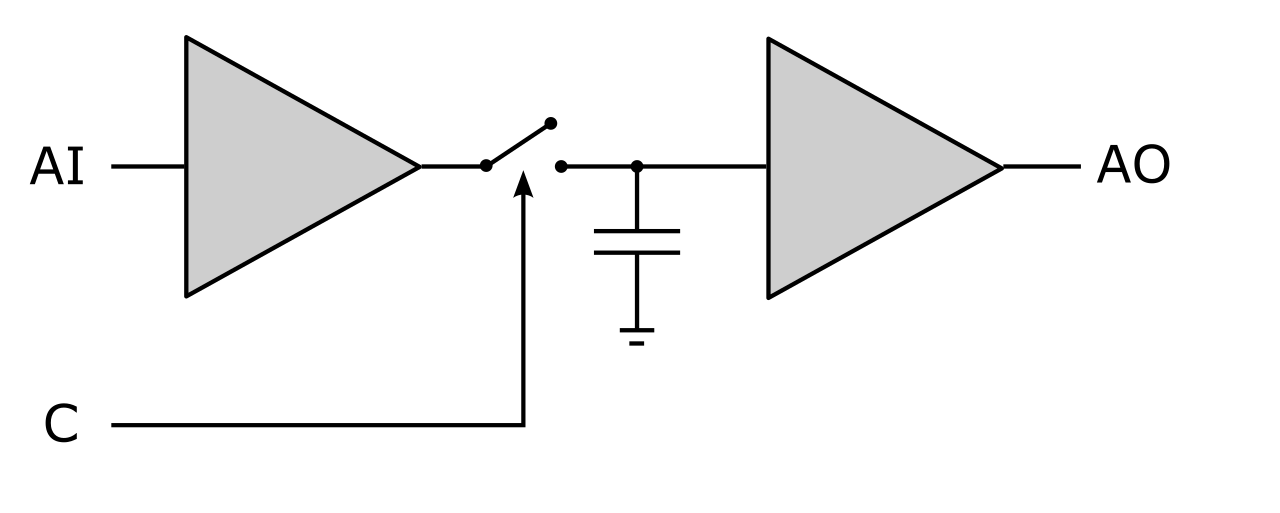
\includegraphics[scale=0.25]{figures/SH}
\caption{A simplified schematic of an S\&H circuit (Source: \href{https://en.wikipedia.org/wiki/File:Sample-hold-circuit.svg}{Wikipedia})}
\label{fig:SH}
\end{figure}
\newpar
A common way of stabilizing the in- and outputs of many of these converters is to use a \tbf{Sample \& Hold Circuit}, which uses a capacitor to charge up to an input voltage as fast as possible, and then maintain that voltage for a specified amount of time. A simplified schematic of such a circuit can be seen in \ref{fig:SH}.
%
\clearpage
\subsection{Signal Theory}
\tbf{Aliasing} is a process where high-frequency information in an image is mistakenly interpreted as a lower frequency. For a given sampling rate $f_s$, two frequencies $f$ and $f'$ are aliases of each other, meaning that $f'$ will be mistaken for $f$, if $f' = f + k \cdot f_s$ for some integer $k$.
\newpar
The \tbf{Nyquist–Shannon sampling theorem} \footnote{Actually first discovered by by E. T. Whittaker in 1915, and thus also known as the \textit{Whittaker–Shannon sampling theorem, Whittaker–Shannon theorem}, or \textit{Whittaker–Nyquist–Shannon theorem}. It is sometimes also simply called the \textit{cardinal theorem of interpolation}.} states that aliasing occurs when the sampling frequency $f_s$ is lower than the maximum input frequency $f_b$ multiplied by $2$, and therefore a signal must be sampled at $f_s \geq 2f_b$ to get an accurate result\footnote{Shannon's original version only stated \textit{``If a function $x(t)$ contains no frequencies higher than $B$ hertz, then it can be completely determined from its ordinates at a sequence of points spaced less than $\frac{1} {2B}$ seconds apart.''}}.
\newpar
\tbf{Baseband sampling} occurs when all signals of interest lie within the \tbf{Nyquist Bandwidth}, i.e. they are all smaller than $\frac{1}{2}f_s$. In this case, we need to filter out aliases at higher frequencies.
\newpar
\tbf{Undersampling} occurs when images between $\frac{1}{2}f_s$ and $f_s$ are sampled. In the case of undersampling, the first Nyquist zone (the interval $[0, \frac{1}{2}f_s]$) contains aliases of the same signals in frequency-reversed order. This means that, if there is also a known lower bound $f_a$ on the input frequencies, then we can clearly identify the high-frequency signals through their aliases in the first Nyquist zone, meaning that \tbf{if we want to measure a signal of bandwidth $\Delta f$, then it is enough to sample at $f_s \geq 2 \Delta f$}. An equivalent statement is that \tbf{if we want to sample a signal whose frequencies are known to lie between $f_a$ and $f_b$, then it is enough to sample at $f_s \geq 2(f_b - f_a)$}.
\chapter{Software}
\thispagestyle{fancy}
A big software chapter was teased all throughout the lecture but besides a non-exam-relevant chapter on the very very basic basics of embedded AI it was basically skipped :\textsuperscript{$\wedge$})
%
\appendix
\chapter{Sources}
\thispagestyle{fancy}
The content of these notes primarily comes from the slides provided by Prof. Amft and Lars Häusler.
\newpar
Additional sources include \href{http://www.en.wikipedia.org}{Wikipedia} for theoretical topics and \href{http://www.vhdlwhiz.com}{vhdlwhiz.com}, \href{http://www.vhdl-online.de}{vhdl-online.de} and \href{https://www.sigasi.com/tech/}{sigasi.com} for VHDL.
\newpar
A tool of dubious quality that was nevertheless used frequently throughout the lecture for playing around with VHDL was \href{https://www.edaplayground.com}{edaplayground.com}.
\newpar
Most of the explanations of petri nets (and state charts) given by the lecture was pretty awful, I found \href{https://www7.in.tum.de/~esparza/fcbook-middle.pdf}{\textit{``Free Choice Petri Nets''} by Jörg Desel and Javier Esparza} to be a helpful resource in properly explaining properties like liveness or deadlock-freeness. Most of the other content of the lecture was very badly presented too, but at least for those it was either easy to deduce correct definitions from the unclear/informal/wrong definitions given on the slides. The signal processing theory chapter was also really really bad though, but thankfully, unlike for petri nets, information on signal processing is readily available on wikipedia. =w=
\end{document}
